\documentclass{article}

\usepackage{amsmath}
\usepackage[margin=1in]{geometry}
\usepackage{graphicx}

\newcommand{\code}{\texttt}
\newcommand{\pkg}{\textbf}

\setlength{\parindent}{0in}

\begin{document}


\section*{How many of each cause of homicide?}

First download the \code{Baltimore\_homicides.zip} file from
Courseplus and unzip it into your working directory. You can read the
file \code{homicides.txt} with \code{readLines} via
\begin{verbatim}
homicides <- readLines("homicides.txt")
\end{verbatim}
The goal of this exercise is to count the number of different types of
homicides are in this dataset. In each record there is a field with
the word ``Cause'' in it indicating the cause of death (e.g. ``Cause:
shooting''). Try to extract this field and count the number of
instances of each cause.\\

The answer should look something like
\begin{verbatim}
asphyxiation  blunt force        other     shooting     stabbing      unknown 
          28           77            6         1003          121           10 
\end{verbatim}


\section*{Age distribution of homicide victims}

The goal of this part is to make a histogram of the age distribution
of the homicide victims in the dataset. For most (but not all) records
there is an indication of the age of the victim, however it is not
always consisten. Extract the age of the victim using a regular
expression and make a histogram of the ages. It should look something
like the following:
\begin{figure}[h]
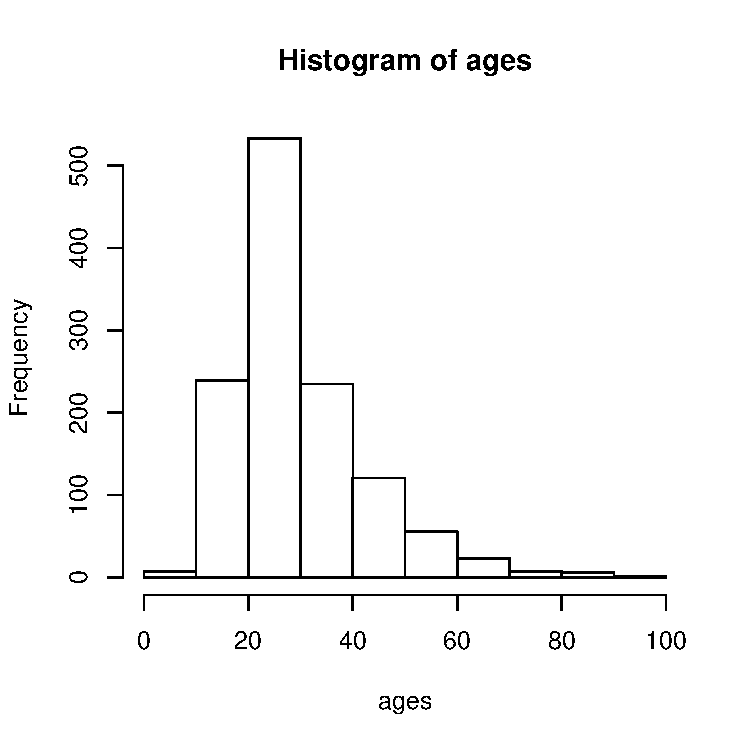
\includegraphics{homicide-ages}
\end{figure}


\end{document}
